\section{Nuclear Physics}

\subsection{nuclear energy}

\subsubsection{mass-energy equivalence}

mass-energy equivalence principle states that mass and energy are equivalent to one another

this idea is represented mathematically by \keypoint{Einstein's mass-energy relation}\index{mass-energy relation}: $\boxed{E=mc^2}$
\footnote{This might be the most famous equation in all physical sciences. When Albert Einstein wrote down the theory of \emph{special relativity} in 1905, he found the mass $m$ of an object with rest mass $m_0$ is related to the speed $v$ at which it is moving by: $m=m_0 \left(1-\frac{v^2}{c^2}\right)^{-\frac{1}{2}}$. Total energy is given by $E=mc^2=m_0 c^2 \left(1-\frac{v^2}{c^2}\right)^{-\frac{1}{2}}$. At low speeds $v \ll c$, $E \approx m_0 c^2 \left(1+\frac{1}{2}\frac{v^2}{c^2}\right) = m_0 c^2 + \frac{1}{2}m_0 v^2$. The second piece clearly gives the kinetic energy term, so the first piece can be thought as the rest energy stored within the mass. This is how the idea of mass-energy relation came to the great mind of Einstein.}

$m$ is \keypoint{rest mass} of the object, $c = 3.00\times10^8 \mps$ is speed of light in vacuum

\cmt mass-energy equivalence implies mass can be converted into pure energy

conversely, mass can be created out of energy

\cmt $\Delta E = \Delta m c^2$ applies to \emph{all} energy changes

if energy is supplied to a system, then mass of this system increases

for example, an object will have a greater mass when it is set to motion or is heated

mass is not a converved quantity, it is \emph{mass-energy} that is conserved in all processes

\cmt if an object is stationary, its mass is called the \emph{rest mass} $m_0$

mass-energy equivalence implies an object at rest still has an intrinsic \emph{rest energy}: $E_0 = m_0 c^2$

\cmt energy transformations such as chemical reactions can cause a system to lose some mass content, but this change in mass is usually negligible

\newpage

\example{When an antiproton (antiparticle of a proton) collides with a proton, they are annihilated and two photons of equal energy are formed. (a) What is the energy of each photon? (b) What is the photon frequency?}

\sol rest energy of proton becomes photon energy:

{

\centering

$E_\gamma=m_pc^2 = 1.67\times10^{-27} \times (3.0\times10^8)^2 \approx 1.50\times10^{-10} \text{ J}$

}

photon frequency: $f=\frac{E_\gamma}{h} = \frac{1.50\times10^{-10}}{6.63\times10^{-34}} \approx 2.27 \times10^{23} \text{ Hz}\,$ (high-frequency $\gamma$-photon) \eoe

\question{The combustion of one mole of solid carbon to form carbon dioxide (CO$_2$) at standard condition is 394 kJ. Find the change in mass for this amount of energy, and hence compare this mass change with the mass of carbon before combustion.}

\question{Given that the specific heat capacity of copper is $380\jpkgk$. When a copper block is heated from 300 K to 1000 K, what is the additional mass as a fraction of its rest mass?}



\subsubsection{binding energy}

\emph{nucleons} (protons and neutrons) in a nucleus bind together through the \emph{strong nuclear force}

to pull nucleons apart, work must be done to overcome the attraction

so free nucleons at infinity have greater potential energy than a single nucleus

since energy is equivalent to mass, free nucleons would appear more massive than when they are held together in a nucleus

this statement is supported by experimental data

useful notions in nuclear physics related to this idea can now be introduced

\begin{ilight}
	difference between mass of a nucleus and total mass of its constituent nucleons when separated to infinity is called the \keypoint{mass defect}\index{mass defect}
\end{ilight}

\begin{ilight}
	energy needed to separate the nucleons in a nucleus to infinity, or equivalently, energy released when free individual nucleons combine to form a nucleus, is called the \keypoint{nuclear binding energy} ($E_B$)\index{binding energy}
\end{ilight}

\cmt for a nucleus $Z$ with proton number $Z$ and nucleon number $A$ (represented by $^A_Z X$)

its mass defect is given by: $\Delta m = Z \Mp + (A-Z)\Mn -m_X$

where $\Mp = 1.673 \times 10^{-27} \text{ kg}$ is mass of proton, $\Mn = 1.675 \times 10^{-27} \text{ kg}$ is mass of neutron

\cmt by definition, binding energy is equivalent to mass defect: $\boxed{E_B = \Delta m c^2}$

\cmt nucleons in a nucleus have \emph{negative} P.E., while free  nucleons have zero P.E.

$E_B$ is the energy required to fill this gap in order to pull nucleons apart

i.e., $E_B$ of a nucleus equals \emph{loss} of potential energy during its formation

\cmt nuclear mass is often measured in \emph{unified atomic mass} u, where $\boxed{1 \text{ u} = 1.66\times10^{-27} \text{ kg}}$

nuclide $^A_Z X$ has a nuclear mass of about $A\text{u}$

\cmt binding energy is often measured in MeV, where $\boxed{1 \text{ MeV} = 10^6 \text{ eV} = 1.60\times10^{-13} \text{ J}}$ 

\example{An iron-56 nucleus ($^{56}_{26}$Fe) has a mass of $9.288 \times 10^{-26} \text{ kg}$. Calculate the nuclear binding energy per nucleon, in MeV, for $^{56}_{26}$Fe.}

\sol mass defect: $\Delta m = 26m_\text{p} + (56-26)m_\text{n} - m_\text{Fe} = 26\times 1.673\times10^{-27} + 30 \times1.675\times10^{-27} - 9.288 \times 10^{-26}$

so we find $\Delta m = 8.68 \times 10^{-28} \text{ kg}$

binding energy: $E_B = \Delta m c^2 = 8.68 \times 10^{-28} \times (3.00\times10^8)^2 \approx 7.812 \times 10^{-11} \text{ J}$

binding energy per nucleon: $\epsilon_b = \frac{E_b}{A} = \frac{7.812 \times 10^{-11}}{56} \approx 1.395 \times 10^{-12} \text{ J}$

\eqyskip convert into MeV: $\epsilon_b = \frac{1.395 \times 10^{-12}}{1.60\times10^{-13}} \text{ MeV} \approx 8.72 \text{ MeV}$ \eoe

\question{Show that the energy equivalent of 1.0 u is 934 MeV.}

\question{Given that mass of proton is 1.007 u, mass of neutron is 1.009 u, and mass of uranium-235 nucleus is 234.992 u. Find the binding energy per nucleon of nuclide $^{235}_{\phantom{2}92}\text{U}$.}

\question{What is the binding energy for the hydrogen nucleus $^1_1\text{H}$?}

\question{Why is rest mass of proton slightly larger than the unified atomic mass unit?}

\subsubsection{nuclear stability}

binding energy per nucleon $\epsilon_b$ is closely related to nuclear stability

binding energy per nucleon gives average energy needed to remove a nucleon from nucleus

higher $\epsilon_b$ means more difficult to pull nucleons away, so nucleus has higher stability

a graph of $\epsilon_b$ against nucleon number $A$ can be plotted based on experimental data

\begin{figure}[ht]
\centering
\begin{tikzpicture}[scale=0.92]
\draw[thick,<->] (0,9.5*.75) node[left]{$\epsilon_b$/MeV} -- (0,0) -- (250*.045,0) node[below]{$A$};
\foreach \A in {0,50,...,200} \draw[thick] (\A*0.045,0) node[below]{\A} --++ (0,0.1);
\foreach \eb in {0,1,...,9} \draw[thick] (0,\eb*0.75) --++ (-0.1,0) node[left]{\eb};
\draw plot[mark=triangle*, mark options={fill=white}] file {nuclearBE.data};
\draw [very thick,->,purple](1,2) [out=90,in=250] to (1.4,5);
\node[right] at (1.1,3.5){fusion};
\draw [very thick,->,purple] (10,5) -- (5,5.6);
\node[below] at (7.5,5.2) {fission};
\draw plot[mark=triangle*, mark options={fill=red}] (56*.045,8.790*.75);
\node[red,above] at (56*.045,8.9*.75) {$^{56}_{26}$Fe};
\end{tikzpicture}

\caption*{binding energy per nucleon $\epsilon_b$ against nucleon number $A$}

\vspace*{-12pt}
\end{figure}


\cmt $^{56}_{26}$Fe has greatest value of $\epsilon_b$ for all nucleus $\ra$ $^{56}_{26}$Fe is the most stable nuclide in nature

\cmt any physical system would evolve such that it lowers total energy

if there could be an increase in total binding energy, nuclear reactions could occur


\subsubsection{fusion}

for nuclei smaller than $^{56}_{26}$Fe, they could combine together and release energy

\begin{ilight}
	\keypoint{fusion}\index{fusion} is the process where two light nuclei join together to form a heavier nucleus
\end{ilight}

\cmt fusion occurs only at very \emph{high temperatures}

nuclei are all positively charged, for two nuclei to come close enough to fuse together, high initial K.E. is needed for them to overcome their \emph{electrostatic repusion}

\cmt vast amount of energy of the sun and other \emph{stars} are created through fusion

extreme high temperature and high density at core of stars make fusion possible
\footnote{Even for the simplest fusion reaction, fusing hydrogen into helium, at least $1.5\times 10^7 \text{ K}$ is required. This is basically how the sun shines and nurtures lives on the earth, and also many other stars in the universe power energies. For a sufficiently massive star, when it burns out of its fuel, its core collapses and becomes hot enough to start to fuse heavier elements. If a star is not able to fuse again, nuclear reaction ceases, the star collapses and becomes a \emph{white dwarf}. For a giant star, nuclear reactions can go all the way up to $^{56}_{26}$Fe. At this point, no more energy can be produced through fusion. The star collapses extremely rapidly and then explodes, creating a \emph{supernova}, during which all elements heavier than $^{56}_{26}$Fe are formed. ($\ast$)}


\subsubsection{fission}

for a nucleus larger than $^{56}_{26}$Fe, it can break into two or more parts and release energy

\begin{ilight}
	\keypoint{fission}\index{fission} is the process where a massive nucleus splits into two smaller nuclei of about the same size (and is usually associated with release of several neutrons)
\end{ilight}

\cmt note that fission requires the two product nuclei are of simliar size

$\alpha$-decay (emission of helium necleus from an unstable nucleus) is not a fission process

\cmt fission reactions can occur \emph{spontaneously}, i.e. nuclei can undergo fission by themselves

fission can also be \emph{induced} by bombarding the nucleus with an incident neutron

induced fission is used by humans to generate nuclear power or to build nuclear weapons

\subsubsection*{nuclear reactors ($\ast$)}

nuclear reactors make use of energy released from induced fission reactions

thermal energy produced from fission is further converted to electrical or mechanical forms

uranium-235 ($^{235}_{\phantom{1}92}\text{U}$) is the most widely used fuel for fuel nuclear reactors

one of the many fission reactions of uranium-235 is: $^{235}_{\phantom{1}92}\text{U} + ^1_0\text{n} \longrightarrow  ^{141}_{\phantom{1}56}\text{Ba} + ^{92}_{36}\text{Kr} + 3^1_0\text{n}$

\cmt each reaction releases more than one neutrons

they can trigger further fission reactions, making \emph{chain reaction} possible

hence huge amount of energy can be released in a very short time

\cmt rate of fission should be controlled, a runaway reaction could lead to disastrous explosion

\emph{control rods} (e.g., boron) are used to absorb neutrons: $^{10}_{\phantom{1}5}\text{B} + ^1_0\text{n} \longrightarrow  ^{7}_{3}\text{Li} + ^{4}_{2}\text{He}$

control rods are adjusted so that one neutron per reaction goes on to produce further fission

in emergency, release of boron rods shuts down reactor

\cmt reaction is expected to continue at steady rate

need sufficient amount of neutrons to maintain the chain reaction

this requires a \emph{critical mass} for the amount of $^{235}_{\phantom{1}92}\text{U}$ fuel

\cmt only low energy neutrons (\emph{thermal neutrons}) can be \emph{captured} by $^{235}_{\phantom{1}92}\text{U}$

but neutrons released through fission are very energetic

a \emph{moderator} (e.g., water) is needed to slow down neutrons

\cmt heat produced in fission is removed by \emph{coolant} (e.g., water)

this heat can be used to power generators to produce electricity

\cmt reactor is surrounded by a \emph{shield} (e.g., a thick concrete) to prevent radiation from escaping

\subsubsection{energy release from nuclear reactions}

in this section, we consider only those nuclear reactions that release energy

let's write a generic nuclear reaction as: $\text{original particles} \longrightarrow \text{product particles} + Q$

two approaches to compute $Q$, the amount of energy release, will be introduced

\noindent \textbf{method 1}: use change in \emph{mass} during the reaction

there must be a decrease in total mass to be converted into energy release

using mass-energy relation: $Q=\Delta mc^2 = (m_\text{org} - m_\text{prod})c^2$

\noindent \textbf{method 2}: use change of \emph{total binding energy}

energy is released means product particles are more stable

so total binding energy of product particles is higher than that of original particles

energy released during reaction: $Q= E_{B,\text{prod}} - E_{B,\text{org}}$

\example{The sun is a huge nuclear reactor. It fuses hydrogen nuclei into helium nuclei to produce large amounts of energy. The reaction can be expressed by the formula:}

{

\centering

$4 ^1_1\text{H} \longrightarrow ^4_2\text{He} + 2 ^{\phantom{+}0}_{+1}\text{e} \quad$ ($^{\phantom{+}0}_{+1}\text{e}$ is a \emph{positron}, the anti-particle of electron)

}

\noindent (a) Evaluate the energy released in one reaction. (b) Given that the power output of the sun is roughly $4.0\times10^{26}\text{ W}$, estimate how much hydrogen the sun burns every second. (Data for this question: $m_\text{p}=1.672622\times10^{-27}\text{ kg} \,$, $m_\text{He}=6.644657\times10^{-27}\text{ kg} \,$,  $m_\text{e}=9.11\times10^{-31}\text{ kg}$)


\sol energy released in one reaction:

{
	
	\centering

	$E_0 = \Delta mc^2 = (4m_\text{H} - m_\text{He} - 2m_\text{e}) c^2 \approx 4.40\times10^{-29} \times (3.0\times10^8)^2 \approx 3.96\times10^{-12} \text{ J}$
	
}

in interval $\Delta t$, sun outputs a total energy of $P\Delta t$ via a number of $\Delta N$ fusion reactions

we write $P\Delta t = \Delta N E_0$, so number of fusion reactions every second is:

{
	
	\centering
	
	$\frac{\Delta N}{\Delta t} = \frac{P}{E_0} = \frac{4.0\times10^{26}}{3.96\times10^{-12}} \approx 1.0\times 10^{38} \text{ s}^{-1}$
	
}

each reaction takes four hydrogen nuclei, so rate of hydrogen consumption:

{
	
	\centering
	
	$\frac{\Delta M_\text{H}}{\Delta t} = \frac{4\Delta N}{\Delta t} \times m_\text{H} \approx 4 \times 1.0\times 10^{38} \times1.67\times10^{-27} \approx 6.7\times10^{11} \text{ kg s}^{-1}$
	
}

the sun burns over 600 billion kilograms of hydrogen every second, just think about it! \eoe

\begin{wrapfigure}{r}{0.42\textwidth}
	\vspace*{-21pt}
	\flushright
	\begin{tabular}{|c|c|}
		\hline
		& binding energy per nucleon \\ \hline
		$^{235}_{\phantom{2}92}\text{U}$ & 7.591 MeV \\ \hline $^{141}_{\phantom{1}56}\text{Ba}$ & 8.326 MeV\\ \hline $^{92}_{36}\text{Kr}$ & 8.513 MeV\\ \hline
	\end{tabular}
	\vspace*{-10pt}
\end{wrapfigure}

\example{Uranium-235 nuclei ($^{235}_{\phantom{2}92}$U) bombarded with slow neutrons can undergo nuclear reaction:}
	
{

\centering

$^1_0\text{n} + ^{235}_{\phantom{2}92}\text{U} \longrightarrow ^{141}_{\phantom{1}56}\text{Ba} + ^{92}_{36}\text{Kr} + x^1_0\text{n}$

}

\noindent (a) Determine the number of $x$. (b) Using the data in the table, find the energy released for one reaction. (c) What is the change in mass, if any, before and after the reaction?

\sol from conservation of mass number: $1+235=141+92+x \ra x=3$

energy release during reaction equals change in total binding energy:

{

\centering

$Q=E_{B,\text{Ba}} + E_{B,\text{Kr}} - E_{B,\text{U}} = 141\times8.326+92\times8.513-235\times7.591=173.277 \text{ MeV} $

}

reduction in total mass: $\Delta m = \frac{Q}{c^2} = \frac{173.277\times1.60\times10^{-13}}{(3.0\times10^8)^2} \approx 3.08\time10^{-28} \text{ kg}$ \eoe


\begin{wrapfigure}{r}{0.45\textwidth}
	\vspace*{-21pt}
	\flushright
	\begin{tabular}{|c|c|}
		\hline
		& binding energy per nucleon \\ \hline
		$^{235}_{\phantom{2}92}\text{U}$ & 7.591 MeV \\ \hline $^{144}_{\phantom{1}55}\text{Cs}$ & 8.212 MeV\\ \hline $^{92}_{36}\text{Kr}$ & 8.631 MeV\\ \hline
	\end{tabular}
	\vspace*{-10pt}
\end{wrapfigure}

\question{Uranium-235 nuclei can undergo another fission process when being bombarded with neutrons. This is represented by:}

{
	
	\centering
	
	$^1_0\text{n} + ^{235}_{\phantom{2}92}\text{U} \longrightarrow ^{144}_{\phantom{1}55}\text{Cs} + ^{90}_{37}\text{Rb} + 2^1_0\text{n}$	
	
}

\noindent Calculate the energy released in this reaction.


\begin{wrapfigure}{r}{0.2\textwidth}
	\vspace*{-21pt}
	\flushright
	\begin{tabular}{|c|c|}
		\hline
		& mass/u \\ \hline
		$^1_1\text{H}$ & 1.00728 \\ \hline
		$^2_1\text{D}$ & 2.01356 \\ \hline 
		$^3_2\text{He}$ & 3.01605 \\ \hline
	\end{tabular}
	\vspace*{-10pt}
\end{wrapfigure}



\question{The \emph{proton–proton chain reaction} is a set of nuclear reactions through which stars fuse hydrogen into helium. One intermediate reaction may be summarised as:	}

{

\centering

$ ^1_1\text{H} + ^2_1\text{D} \longrightarrow ^3_2\text{He} + \text{energy}$

}
	
\noindent Calculate the energy released in this reaction.


\question{Another fusion reaction in the proton-proton chain is represented by:}

{
	
	\centering

	$^3_2\text{He} + ^3_2\text{He} \longrightarrow ^4_2\text{He} + 2 ^1_1\text{p} +\text{energy}$	
	
}

\noindent where energy released through this reaction is 12.86 MeV. Given that binding energy per nucleon of $^4_2\text{He}$ is 7.074 MeV, calculate the binding energy per nucleon for $^3_2\text{He}$.

\question{If the total mass of the product particles is greater than that of the original particles in a nuclear reaction, what can you say about the energy of the original particles?}




\subsection{radioactive decay}

\subsubsection{radioactive decay}

\rcyskip

\begin{ilight}
	the process of \emph{random} and \emph{spontaneous} emission of $\alpha$-, $\beta$-, and $\gamma$-radiation from unstable nuclei is called \keypoint{radioactive decay}\index{radioactive decay}
\end{ilight}

\cmt \keypoint{random} means decay events are not predictable

we cannot tell precisely when a particular nucleus is about to decay

we can only tell the \emph{probability} of decay within a certain time

\cmt \keypoint{spontaneous} means rate of decay does not depend on external conditions

temperature, pressure, or has no effect on rate of radioactive decays

\vspace*{\baselineskip}

suppose initially a sample contains $N$ radioactive nuclei that are about to decay

after a time interval $\Delta t$, $\Delta N$ nuclei undergo decay processes

probability of decay for nuclei in the sample during this time interval is $\frac{\Delta N}{N}$

divide by $\Delta t$, probability of decay for each nucleus per unit time can be found

since nuclear decay is spontaneous, this number is a constant, called the decay constant

\begin{ilight}
	\keypoint{decay constant}\index{decay constant} is the probability for one nucleus to decay per unit time: $\boxed{\lambda = \frac{\Delta N}{N\Delta t}}$
\end{ilight}

\cmt to describe the rate of decay, we introduce the notion of \keypoint{activity}\index{activity}

activity is defined as the number of nuclei that undergo decay per unit time: $\boxed{A=\frac{\Delta N}{\Delta t}}$

this can be given in a differential form: $A = - \frac{\dd N}{\dd t}$

a minus sign is included because number of nuclei $N$ decreases with time

\cmt compare with the expression for decay constant, we find: $\boxed{A=\lambda N}$

this equation shows that if there are more nuclei present, the sample has greater activity

\cmt units for decay constant and activity: $[\lambda] = [A] = \text{s}^{-1}$

for activity, one decay event per unit time is defined as one \emph{becquerel}: $1 \text{ Bq} = 1 \text{ s}^{-1}$



\subsubsection{decay equations}

variation of number of undecayed nuclei with time can be derived from the equation: $A=\lambda N$

recall that $A = - \frac{\dd N}{\dd t}$, so this equation is a differential equation in disguise: $- \frac{\dd N}{\dd t} = \lambda N$

this can be solved by separating variables and integrating

{

\centering

$- \lambda \dd t = \frac{\dd N}{N} \ra
- \lambda \int_0^t \dd t = \int_{N_0}^{N} \frac{\dd N}{N} \ra
- \lambda t \Big|_{0}^{t}= \ln N \Big|_{N_0}^{N} \ra
- \lambda t = \ln \frac{N}{N_0} \ra
N = N_0 \mathrm{e}^{- \lambda t}$

}

this shows that decay events obey \emph{exponential decay laws}

\cmt number of undecayed nuclei at time $t$ is given by: $\boxed{N(t)=N_0 \mathrm{e}^{- \lambda t}}$

$N_0$ is initial number of nuclei in the sample at $t=0$

\cmt $\lambda \up \ra$ higher probability of decay, or greater rate of decay

\begin{figure}[ht]
	\centering
	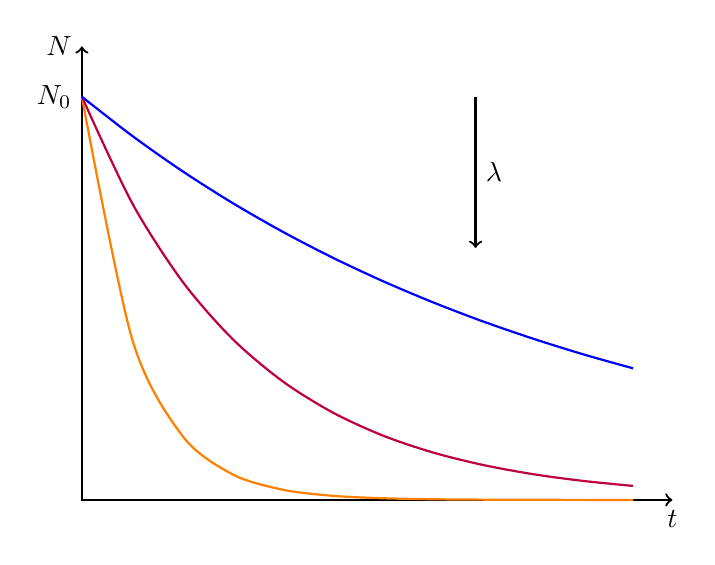
\begin{tikzpicture}[yscale=1.6,xscale=1.25]
	\draw[thick,<->] (0,3.6) node[left]{$N$} -- (0,3.2) node[left]{$N_0$} -- (0,0) -- (6,0) node[below]{$t$};
	\draw[thick,->] (4,3.2) --++ (0,-1.2) node[midway,right]{$\lambda \up$};
	\draw [thick,color=orange,domain=0:5.6,samples=12,smooth,variable=\x] plot (\x,{3.2*exp(-1.8*\x)});
	\draw [thick,color=purple,domain=0:5.6,samples=12,smooth,variable=\x] plot (\x,{3.2*exp(-0.6*\x)});
	\draw [thick,color=blue,domain=0:5.6,samples=12,smooth,variable=\x] plot (\x,{3.2*exp(-0.2*\x)});
	\end{tikzpicture}
	
	\caption*{exponential decay law for number of nuclei: $N(t)=N_0\mathrm{e}^{-\lambda t}$}
	\vspace*{-12pt}
\end{figure}

\cmt since activity $A=\lambda N$, so activity varies with time as: $\boxed{A(t) = A_0 \mathrm{e}^{- \lambda t}}$





\example{A sample containing $6.0\times10^7$ iodine-131 nuclei has an activity of 60 Bq. (a) What is the decay constant of iodine-131? (b) How many nuclei remain undecayed after 20 days?}

\sol decay constant: $\lambda = \frac{A}{N} = \frac{60}{6.0\times10^7} \approx 1.0 \times 10^{-6} \text{ s}^{-1}$

number of remaining nuclei: $N=N_0 \mathrm{e}^{-\lambda t} = 6.0\times10^7 \times \mathrm{e}^{-1.0 \times 10^{-6} \times20\times24\times3600} \approx 1.1\times10^7$ \eoe

\example{$^{24}_{11}\text{Na}$, an isotope of sodium, has a decay constant of $1.28\times10^{-5} \text{ s}^{-1}$. Suppose a sample initially contains a mass of 9.0 $\mu\text{g}$ of $^{24}_{11}\text{Na}$. Find (a) initial number of $^{24}_{11}\text{Na}$ nuclei, (b) initial activity of this sample, (c) the activity after 48 hours.}

\sol initial number of nuclei: $N_0 = \frac{9.0 \text{ }\mu\text{g}}{24\text{u}} =  \frac{9.0\times10^{-9}}{24\times1.66\times10^{-27}} \approx 2.26\times10^{17}$

initial acitivy: $A_0 = \lambda N_0 = 1.28\times10^{-5} \times 2.26\times10^{17} \approx 2.89\times10^{12} \text{ Bq}$

activity after 20 hours: $A=A_0\mathrm{e}^{-\lambda t} = 2.89\times10^{12} \times \mathrm{e}^{-1.28\times10^{-5} \times48\times3600} \approx 3.17\times10^{11} \text{ Bq}$ \eoe

\question{A sample of polonium-205 has an activity of $6.7\times10^{15}$ Bq. The decay constant of polonium-205 is known to be $1.16\times10^{-4} \text{ s}^{-1}$. (a) Find the number of nuclei needed to give this activity. (b) Find the mass of polonium-205 in this sample. (c) Calculate the time needed for the activity reduce to 1\% of its initial value.}

\question{Technetium-99m is widely used as a radioactive tracer for medical diagnostic procedures. If some of this isotope, with an activity of 900 MBq was injected into a patient. The activity is found to reduce to 56.4 MBq after 24 hours. (a) What is the decay constant of technetium-99m? (b) How many technetium-99m nuclei are stil left in the patient's body?}


\subsubsection{half-life}

it is more convenient to define a time quantity to describe how fast radioactive nuclei decay

it is useful to define half-life  of a radioactive sample
 
\begin{ilight}
	\keypoint{half-life}\index{half-life} ($\halflife$) is the mean time taken for number of radioactive nuclei in the sample, or activity of the sample, to reduce to half of its initial value
\end{ilight}

\cmt half-life $\halflife$ is closely related to decay constant $\lambda$

by definition, at $t=\halflife$, $N=\frac{1}{2}N_0$, $A=\frac{1}{2}A_0$ $\RA \mathrm{e}^{- \lambda \halflife} = \frac{1}{2} \RA \mathrm{e}^{\lambda \halflife} = 2 \RA \boxed{\lambda \halflife= \ln 2}$

\cmt $\lambda$ is a constant, so $\halflife$ is also a constant over the lifetime of nuclear decay

half-life of a sample of isotope does not depend on initial number of nuclei or initial activity

\begin{figure}[ht]
	\centering
	\begin{tikzpicture}[yscale=1.6,xscale=1.35]
	\draw[thick,<->] (0,3.6) node[left]{\large \sfrac{$N$}{$N_0$}} -- (0,3.2) node[left]{$1$} -- (0,0) -- (6,0) node[below]{$t$};
	\draw [thick,color=blue,domain=0:5.6,samples=12,smooth,variable=\x] plot (\x,{3.2*exp(-0.4*\x)});
	\draw[thick,dashed] (0,1.6) node[left]{\large \sfrac{1}{2}} -- ++ ({2.5*ln(2)},0) -- ++ (0,-1.6);
	\draw[thick,dashed] (0,0.8) node[left]{\large \sfrac{1}{4}} -- ++ ({5*ln(2)},0) -- ++ (0,-0.8);
	\draw[thick,dashed] (0,0.4) node[left]{\large \sfrac{1}{8}} -- ++ ({7.5*ln(2)},0) -- ++ (0,-0.4);
	\node[below] at (0,0) {0};
	\node[below] at ({2.5*ln(2)},0) {$\halflife$};
	\node[below] at ({5*ln(2)},0) {2$\halflife$};
	\node[below] at ({7.5*ln(2)},0) {3$\halflife$};
	\end{tikzpicture}
	
	\caption*{half-life of radioactive decay}
	\vspace*{-12pt}
\end{figure}

\example{Radium-224 has a half-life of 3.63 days. (a) What is the activity from 6.0 mg of pure radium-224? (b) How many radium-224 nuclei have undergone decay after 10 days?}

\sol decay constant: $\lambda = \frac{\ln 2}{\halflife} = \frac{\ln 2}{3.63\times24\times3600} \approx 2.21\times10^{-6} \text{ s}^{-1}$

\eqyskip initial number of Ra-224 nuclei: $N_0 = \frac{6.0 \text{ mg}}{224 \text{ u}} = \frac{6.0\times10^{-6}}{224\times1.66\times10^{-27}} \approx 1.61\times10^{19}$

initial acitivy: $A_0 = \lambda N_0 = 2.21\times10^{-6} \times 1.61\times10^{19} \approx 3.57\times10^{13} \text{ Bq}$

number of undecayed nuclei: $N=N_0\mathrm{e}^{-\lambda t} = 1.61\times10^{19} \times \mathrm{e}^{-2.21\times10^{-6}\times10\times24\times3600} \approx 2.39\times10^{18}$

number of nuclei that have decayed: $\Delta N = N_0 - N = 1.61\times10^{19} - 2.39\times10^{18} \approx 1.37\times10^{19}$ \eoe

\example{Living trees contain a certain percentage of $^{14}_{\phantom{1}6}\text{C}$, an radioactive isotope of carbon that has a half-life of 5570 years. A sample of dead wood is found to have an activity of 0.42 Bq, while an equal mass of living wood has an activity of 1.60 Bq. Find the age of the dead wood.}

\solc\begin{equation*}
	A=A_0\mathrm{e}^{-\lambda t} = A_0\mathrm{e}^{ -\frac{\ln 2}{\halflife} t} \ra 0.42 = 1.60 \mathrm{e}^{ -\frac{\ln 2}{5570} t} \ra -\frac{\ln 2}{5570} t = \ln\left(\frac{0.42}{1.60}\right) \ra t\approx 10700 \text{ years} \teoe
\end{equation*}

\question{The number of uranium-238 nuclei in a rock sample is believed to have decreased from $3.50\times10^{17}$ to $3.27\times10^{17}$ in 480 million years.	Estimate the half-life of uranium-238.}

\question{Plutonium-238 is a powerful alpha emitter with a half-life of 87.7 years. One decay of plutonium-238 releases an energy of about $9.0\times10{-13}$ J. A nuclear battery containing a sealed plutonium source is implanted into patient's body to power heart pacemakers. The battery has an initial activity of $6.0\times10^{10}$ Bq. (a) Calculate the initial power released by the source. (b) Find the mass of plutonium required to produce this power. (c) It is required that power output to the pacemaker is at least 60\% of the initial power. Calculate the time, in years, for which the battery provides sufficient power.}

\question{Show that the variation of the number of undecayed nuclei with time $t$ can be given by: $N(t) = N_0 \left(\frac{1}{2}\right)^{\frac{t}{\halflife}}$, where $N_0$ is the initial number of nuclei.}


\subsubsection{measurement of radioactive decay}

\begin{wrapfigure}{r}{0.45\textwidth}
	\centering
	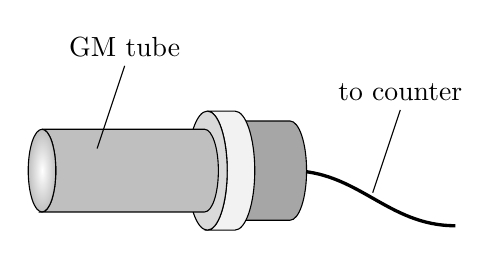
\begin{tikzpicture}[scale=0.7]
	\draw[very thick] (0,0) [out=0, in=180] to (3,-1);
	\draw[fill=gray!70] (-1,.9) -- (0,0.9) arc(90:-90:0.3 and 0.9) -- (-1,-0.9) arc(-90:90:0.3 and 0.9);
	\draw[fill=gray!10] (-1.5,1.08) -- (-1,1.08) arc(90:-90:0.36 and 1.08) -- (-1.5,-1.08) arc(-90:90:0.36 and 1.08);
	\draw[fill=gray!30] (-1.5,0) ellipse (0.36 and 1.08);
	\draw[fill=gray!50] (-4.5,0.75) -- (-1.55,0.75) arc(90:-90:0.25 and 0.75) -- (-4.5,-0.75) arc(-90:90:0.25 and 0.75);
	\shade[draw,shading=radial, inner color=white, outer color=gray!50] (-4.5,0) ellipse (0.25 and 0.75);
	\draw (-3.5,0.4) --++ (0.5,1.5) node[above]{GM tube};
	\draw (1.5,-0.4) --++ (0.5,1.5) node[above]{to counter};
	\end{tikzpicture}
\end{wrapfigure}

a Geiger–M\"uller tube, or a \keypoint{GM tube}\index{GM tube}, is a device used to detect ionizing radiation

GM tube measures the number of $\alpha$-particles, $\beta$-particles and $\gamma$-photons arriving per unit time

the number of decays recorded per unit time by GM tube is called the \keypoint{count rate}\index{count rate} $R$

since GM tube only picks up emissions to one particular direction, but a radioactive source emits radiation in \emph{all} directions, so count rate is a fraction of the activity of the sample

activity obeys exponential decay, so we would expect count rate to satisfy: $\boxed{R=R_0\mathrm{e}^{-\lambda t}}$

\subsubsection*{verifying the exponential decay law}

\begin{wrapfigure}{r}{0.45\textwidth}
	\vspace*{-8pt}
	\centering
	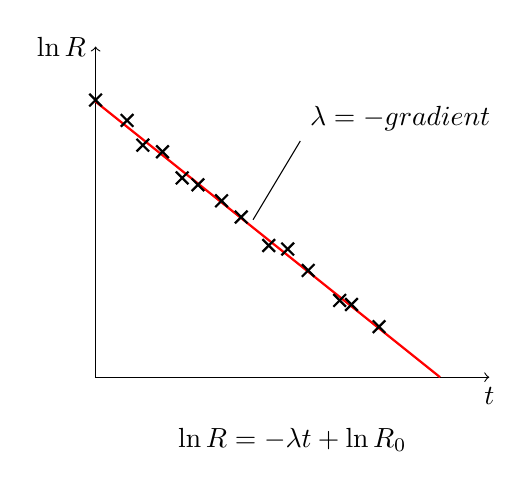
\begin{tikzpicture}
	%\pgfmathsetseed{\number\pdfrandomseed}
	\draw[<->] (0,4.2)node[left]{$\ln R$} -- (0,0) -- (5,0)node[below]{$t$};
	\draw[red,thick] (0,3.5) -- (4.375,0);
	\foreach \x in {0,0.4,0.6,0.85,1.1,1.3,1.6,1.85,2.2,2.44,2.7,3.1,3.25,3.6}{
	\pgfmathsetmacro\somevalue{0.1*rand}
	\draw[thick] (\x-.08,3.58-0.8*\x+\somevalue) --++ (0.16,-0.16);
	\draw[thick] (\x-.08,3.42-0.8*\x+\somevalue) --++ (0.16,0.16);
	}

	\node at (2.5,-0.8) {$\ln R = -\lambda t + \ln R_0$};
	\draw (2,2) -- (2.6,3) node[above right] {$\lambda = -\text{gradient}$};
	\end{tikzpicture}
	\vspace*{-12pt}
\end{wrapfigure}

to verify the exponential decay law, we first rearrange the equation as: $\ln R = -\lambda t + \ln R_0$

if a set of measurements of $R$ at time $t$ are obtained, a graph of $\ln R$ against $t$ can be plotted

if trend curve shows a straight line, the relation $R=R_0\mathrm{e}^{-\lambda t}$ is then verified

decay constant $\lambda$ is given by negative gradient of the best-fit line

\subsubsection*{issues with count rate}

for now, we take for granted that the count rate measured is 100\% accurate

but in practice, there might be a number of factors leading to measurement errors

\begin{compactenum}
	\item[--] there is always \emph{background radiation} from earth minerals, cosmic rays, food and water, etc.
	
	background reading must be subtracted to give a corrected count rate
	
	\item[--] $\alpha$- and $\beta$-particles emitted could be absorbed by sample itself
	
	\item[--] product nuclei could also be radioactive, contributing to additional counts
	
	\item[--] GM tube has \emph{dead time}, or \emph{resolving time}
	
	when a count is recorded, it takes GM tube a certain time
	to reset for the next count
\end{compactenum}

\example{A GM tube is placed close to a source of radioactive isotope. The variation with time $t$ of the measured count rate $R$ is shown. Determine the half-life of this isotope.}

\begin{figure}[ht]
	\centering
	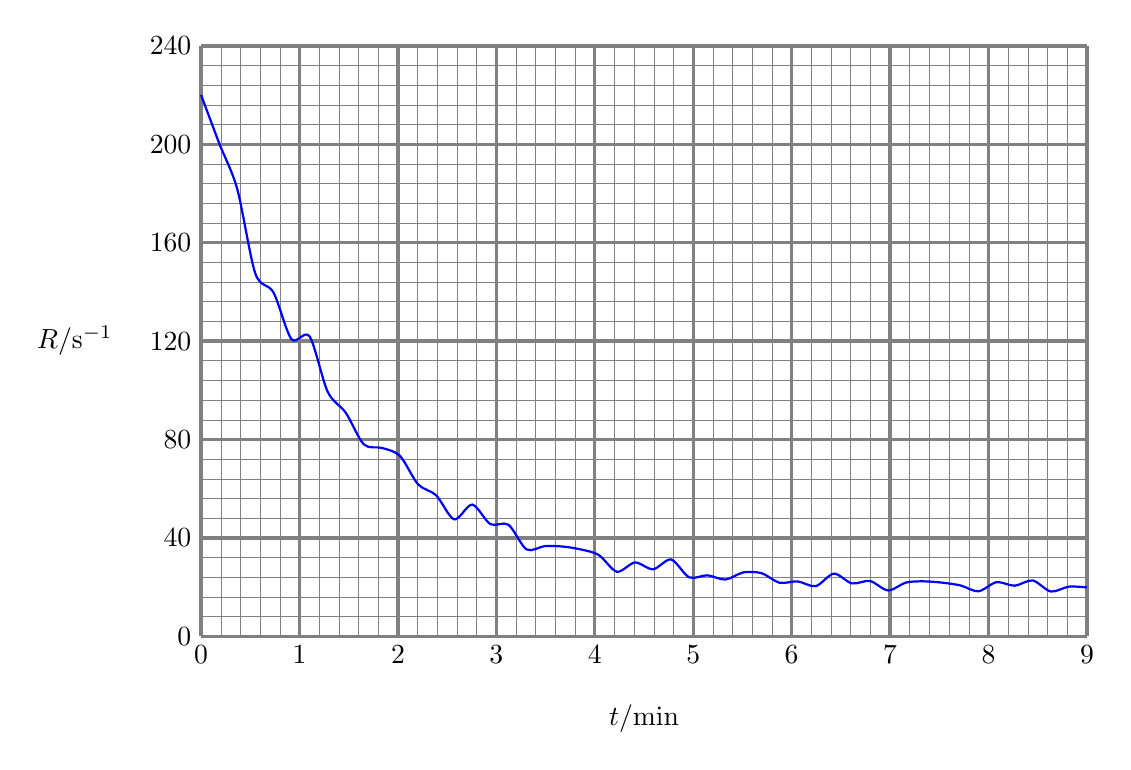
\begin{tikzpicture}[scale=1.25]
	\draw[help lines, very thick] (0,0) grid (9,6);
	\draw[step=0.2, gray, very thin] (0,0) grid (9,6);
	\node[left] at (-0.8,3) {$R$/s$^{-1}$};
	\node[below] at (4.5,-0.6) {$t$/min};
	\foreach \x in {0,1,...,9} \node[below] at (\x,0) {\x};
	\foreach \y in {0,40,...,240} \node[left] at (0,\y/40) {\y};
	\draw [thick,color=blue,domain=0:9,samples=50,smooth,variable=\x] plot (\x,{5.0*exp(-0.7*\x)+0.5+sin(30*\x r)*cos(23*\x r)/(\x+2)*0.75});
	\end{tikzpicture}
\end{figure}

\sol there is evidence of \emph{background radiation} as the count rate decreases and tends to a non-zero value of $20 \text{ s}^{-1}$, so we need subtract this number to obtain the true count rate of sample

there are also \emph{fluctuations} in count rate due to \emph{random} nature of decay processes, so we need to make several calculations and take average to obtain an accurate value for half-life

let's call true count rate $R_T$, and call measured count rate $R$

as $R_T=200 \text{ s}^{-1} \to 100 \text{ s}^{-1}$, $R=220 \text{ s}^{-1} \to 120 \text{ s}^{-1}$, so $\halflife \approx 1.0-0.0 \approx 1.0$ min

as $R_T=160 \text{ s}^{-1} \to 80 \text{ s}^{-1}$, $R=180 \text{ s}^{-1} \to 100 \text{ s}^{-1}$, so $\halflife \approx 1.3-0.4 \approx 0.9$ min

as $R_T=120 \text{ s}^{-1} \to 60 \text{ s}^{-1}$, $R=140 \text{ s}^{-1} \to 80 \text{ s}^{-1}$, so $\halflife \approx 1.6-0.7 \approx 0.9$ min

as $R_T=80 \text{ s}^{-1} \to 40 \text{ s}^{-1}$, $R=100 \text{ s}^{-1} \to 60 \text{ s}^{-1}$, so $\halflife \approx 2.3-1.3 \approx 1.0$ min

take average for these results, we find $\halflife \approx 0.95$ min \eoe
